\documentclass[margin=10pt]{standalone}    

\usepackage{tikz}
\usetikzlibrary{automata, positioning, arrows}

\begin{document}

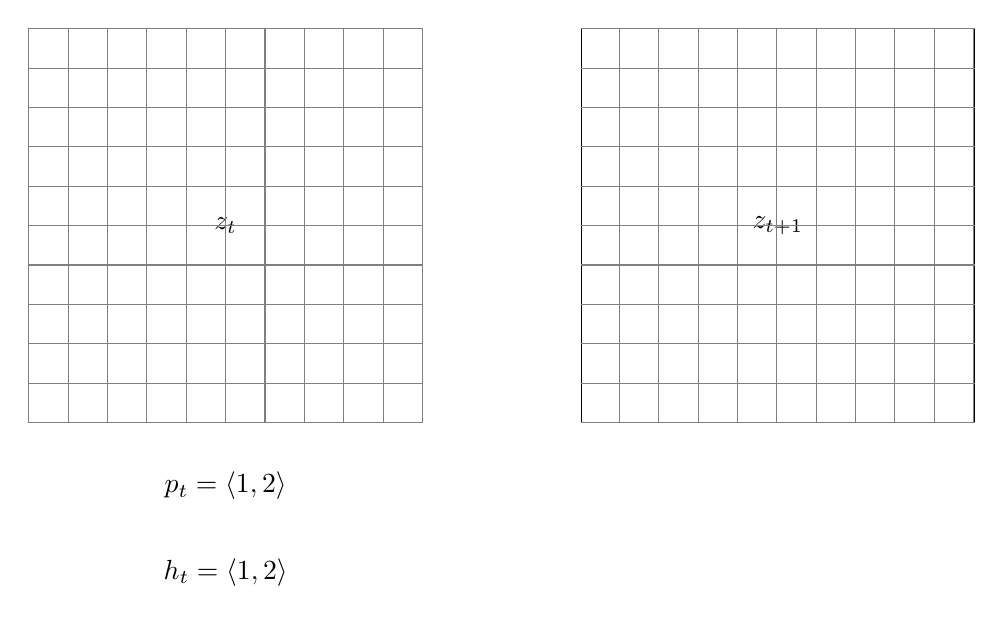
\begin{tikzpicture}[node distance=2cm]
    \tikzstyle{block} = [rectangle,minimum width=5cm,minimum height=5cm,text centered,draw=black,fill=white]
            
    \node (last) [block] {$z_t$};
    \draw [step=0.5,gray,thin] (last.north west) grid (last.south east);

    \node (p) [below=0.5cm of last] {$p_t = \left\langle 1, 2 \right\rangle$};
    \node (h) [below=0.5cm of p] {$h_t = \left\langle 1, 2 \right\rangle$};

    \node (next) [block, right=2cm of last] {$z_{t+1}$};
    \draw [step=0.5,gray,thin] (next.north west) grid (next.south east);

\end{tikzpicture}

\end{document}
